\iffalse 
Section  III: Building and Running the Application   

    Chapter 10: Setting Up the Vitis Environment     

    Chapter 11: Build Targets   
        Software Emulation    
        Hardware Emulation    
        System Hardware Target        

    Chapter 12: Building the Host Program
        Compiling and Linking for x86        
        Compiling and Linking for Arm       

    Chapter 13: Building the Device Binary  
        Compiling Kernels with the Vitis Compiler     
        Compiling Kernels with Vitis HLS        
        Linking the Kernels
        Managing Vivado Synthesis and Implementation Results      
        Controlling Report Generation      

    Chapter 14: Packaging the System        
        Packaging for Embedded Platforms        
        Packaging for Data Center Platforms 

    Chapter 15: Output Directories of the v++ Command     

    Chapter 16: Running Emulation      
        Running Emulation Targets 
        Data Center vs. Embedded Platforms       
        QEMU 
        Running Emulation on Data Center Accelerator Cards
        Running Emulation on an Embedded Processor Platform  
        Speed and Accuracy of Hardware Emulation 
        Working with Simulators in Hardware Emulation        
        Working with SystemC Models        
        Using I/O Traffic Generators       

    Chapter 17: Running the Application Hardware Build     


Section  IV: Profiling, Optimizing, and Debugging the Application

    Chapter 18: Profiling the Application       
        Baselining Functionality and Performance
        Enabling Profiling in Your Application  
        Guidance     
        System Estimate Report
        HLS Report   
        Profile Summary Report
        Timeline Trace        
        Waveform View and Live Waveform Viewer  

    Chapter 19: Optimizing the Performance  
        Host Optimization  
        Kernel Optimization
        Topological Optimization

    Chapter 20: Debugging Applications and Kernels   
        Debugging Flows    
        Debugging in Software Emulation      
        Debugging in Hardware Emulation      
        Debugging During Hardware Execution  
        Debugging on Embedded Processor Platforms     
        Example of Command Line Debugging


Section  V: Vitis Environment Reference Materials  

    Chapter 21: Vitis Compiler Command      
        Vitis Compiler General Options 
        --advanced Options    
        --clock Options    
        --connectivity Options
        --debug Options    
        --hls Options      
        --linkhook Options    
        --package Options  
        --profile Options  
        --vivado Options      
        Vitis Compiler Configuration File    
        Using the Message Rule File 

    Chapter 22: emconfigutil Utility        

    Chapter 23: kernelinfo Utility 
        Kernel Definition  
        Arguments 
        Ports     

    Chapter 24: launch_emulator Utility  
        Versal PS and PMC Arguments for QEMU    
        Zynq UltraScale+ MPSoC PS and PMU Arguments for QEMU      
        Zynq-7000 PS Arguments for QEMU      

    Chapter 25: manage_ipcache Utility      

    Chapter 26: package_xo Command 
        RTL Kernel XML File

    Chapter 27: platforminfo Utility        
        Basic Platform Information     
        Hardware Platform Information        
        Interface Information       
        Clock Information  
        Valid SLRs   
        Resource Availability       
        Memory Information    
        Feature ROM Information     
        Software Platform Information        
        Platforminfo for xilinx_zcu104_base_202010_1     

    Chapter 28: xbutil Utility     

    Chapter 29: xbmgmt Utility     

    Chapter 30: xclbinutil Utility 
        xclbin Information    
        Hardware Platform Information        
        Clocks       
        Memory Configuration  
        Kernel Information    
        Tool Generation Information 

    Chapter 31: xrt.ini File       

    Chapter 32: HLS Pragmas 


Section  VI: Using the Vitis Analyzer    

    Chapter 33: Working with Reports        
        Configuring the Vitis Analyzer 

    Chapter 34: Vitis Analyzer GUI and Window Manager    
        Diff Two Text Files
        Compare Two Timeline Trace Reports      
        Cross-Probing between Reports        
        Using the Floating Ruler       

    Chapter 35: Platform and System Diagrams

    Chapter 36: AI Engine Graphs and Arrays       

    Chapter 37: Link Summary: Multiple Strategies and Timing
        Reports   

    Chapter 38: Setting Guidance Thresholds       

    Chapter 39: Creating an Archive File 


Section  VII: Using the Vitis IDE        

    Chapter 40: Vitis Command Options    

    Chapter 41: Creating a Vitis IDE Project
        Launch a Vitis IDE Workspace   
        Create an Application Project        
        Understanding the Vitis IDE 
        Adding Sources        
        Working in the Project Editor View      
        Working in the Assistant View        
        Output Directories from the Vitis IDE

    Chapter 42: Building the System      
        Vitis IDE Guidance View     
        Working with Vivado Tools from the Vitis IDE     

    Chapter 43: Vitis IDE Debug Flow        
        Using the Standalone Debug Flow
        vitis -debug Command Line   

    Chapter 44: Configuring the Vitis IDE
        Vitis Project Settings
        Vitis Build Configuration Settings      
        Vitis Hardware Function Settings        
        Vitis Binary Container Settings      
        Vitis Toolchain Settings       
        Vitis Run and Debug Configuration Settings       

    Chapter 45: Project Export and Import
        Export a Vitis Project
        Import a Vitis Project
        Import Projects from Git       

    Chapter 46: Getting Started with Examples     
        Installing Examples and Libraries    
        Using Local Copies    

    Chapter 47: RTL Kernel Wizard        
        Launch the RTL Kernel Wizard   
        Using the RTL Kernel Wizard 
        Using the RTL Kernel Project in Vivado IDE    


Section  VIII: Using Vitis Embedded Platforms     

    Chapter 48: Vitis Embedded Platforms    
        Introduction 
        Platform Types        
        Platform Naming Convention     
        Embedded Platform Components and Architecture 
        Installing Embedded Platforms        

    Chapter 49: Using Vitis Embedded Platforms       
        Packaging Images      
        Writing Images to the SD Card        
        Configuring the PL Kernel in DFX Platforms and Non-DFX Platforms   
        Running an Acceleration Application on the Board 
        Software Package Management in PetaLinux rootfs        

    Chapter 50: Creating Embedded Platforms in Vitis 
        Platform Creation Basics       
        Platform Creation Requirements 
        Creating an Embedded Platform        
        Validating an Embedded Platform      
Section  IX: Additional Information      

    Chapter 51: OpenCL Programming 
        OpenCL Host Application     
        OpenCL Kernel Development   

    Chapter 52: Migrating to a New Target Platform   
        Design Migration      
        Migrating Releases    
        Modifying Kernel Placement     
        Address Timing        

    Chapter 53: Legacy Reference   
        xbutil Utility - Legacy     
        xbmgmt Utility - Legacy     

    Chapter 54: Streaming Data Transfers    
        Free-Running Kernel
Section  X: Additional Resources and Legal Notices      
        Xilinx Resources      
        Documentation Navigator and Design Hubs       
        Revision History      
        Please Read: Important Legal Notices    
\fi


%   Section  I: Getting Started with Vitis   
%  The application acceleration development flow is not supported by the Windows OS. 

\section{Introduction to the Vitis Environment for Acceleration} 
\subsection{Accelerated Flow Application Development Using the Vitis Software Platform} 

The Vitis application acceleration development flow provides a framework for developing and delivering FPGA accelerated applications using standard programming languages for both software and hardware components. The software component, or host program, is developed using C/C++ to run on x86 or embedded processors, with OpenCL API calls to manage runtime interactions with the accelerator. The hardware component, or kernel, can be developed using C/C++, OpenCL C, or RTL. The Vitis software platform promotes concurrent development and test of the Hardware and Software elements of an heterogeneous application.

\subsubsection{FPGA Acceleration}
Xilinx FPGAs offer many advantages over traditional CPU/GPU acceleration, including a custom architecture capable of implementing any function that can run on a processor, resulting in better performance at lower power dissipation. When compared with processor architectures, the structures that comprise the programmable logic (PL) fabric in a Xilinx device enable a high degree of parallelism in application execution.

\par To realize the advantages of software acceleration on a Xilinx device, you should look to accelerate large compute-intensive portions of your application in hardware. Implementing these functions in custom hardware gives you an ideal balance between performance and power.

\subsection{Execution Model} 
In the Vitis core development kit, an application program is split between a host application and hardware accelerated kernels with a communication channel between them. The host program, written in C/C++ and using API abstractions like OpenCL, is compiled into an executable that runs on a host processor (such as an x86 server or an Arm processor for embedded platforms); while hardware accelerated kernels are compiled into an executable device binary (.xclbin) that runs within the programmable logic (PL) region of a Xilinx device.


\par The API calls, managed by XRT, are used to process transactions between the host program and the hardware accelerators. Communication between the host and the kernel, including control and data transfers, occurs across the PCIe bus or an AXI bus for embedded platforms. While control information is transferred between specific memory locations in the hardware, global memory is used to transfer data between the host program and the kernels. Global memory is accessible by both the host processor and hardware accelerators, while host memory is only accessible by the host application.

\par The target platform contains the FPGA accelerated kernels, global memory, and the direct memory access (DMA) for memory transfers. Kernels can have one or more global memory interfaces and are programmable. The Vitis core development kit execution model can be broken down into the following steps:

\begin{enumerate}
    \item The host program writes the data needed by a kernel into the global memory of the attached device through the PCIe interface on an Alveo Data Center accelerator card, or through the AXI bus on an embedded platform.
    \item The host program sets up the kernel with its input parameters.
    \item The host program triggers the execution of the kernel function on the FPGA.
    \item The kernel performs the required computation while reading data from global memory, as necessary.
    \item The kernel writes data back to global memory and notifies the host that it has completed its task.
    \item The host program reads data back from global memory into the host memory and continues processing as needed.
\end{enumerate}

The FPGA can accommodate multiple kernel instances on the accelerator, both different types of
kernels, and multiple instances of the same kernel. XRT transparently orchestrates the
interactions between the host program and kernels in the accelerator. 

\subsection{Data Center Application Acceleration Development Flow}
\figref{DataCenterFlow} describes the steps needed to build and run an application for use on the Alveo Data Center accelerator cards.

\begin{enumerate}
    \item x86 Application Compilation: Compile the host application to run on the x86 processor using the G++ compiler to create a host executable file. The host program interacts with kernels in the PL region.
    \item PL Kernel Compilation and Linking: PL kernels are compiled for implementation in the PL region of the target platform. PL kernels can be compiled into Xilinx object form (XO) file using the Vitis compiler (v++), Vitis HLS for C/C++ kernels, or the package\_xo command for RTL
    kernels. 
    \begin{itemize}
        \item The Vitis compiler also links the kernel XO files with the hardware platform to create a device executable (.xclbin) for the application.
        \item Xilinx object (XO) files are linked with the target hardware platform by the v++ --link command to create a device binary file (.xclbin) that is loaded into the Xilinx device on the target platform.
    \end{itemize}

    \item Running the Application: For Alveo Data Center accelerator cards, the .xclbin file is the required build object for running the system. When running the application, you can run software emulation, hardware emulation, or run on the actual physical accelerator platform.

    \begin{itemize}
        \item When the build target is software or hardware emulation, the emconfigutil command builds an emulation model of the target platform. The Vitis compiler generates simulation models of the kernels in the device binary and running the application runs this model of the system. Emulation targets let you build, run, and iterate the design over relatively quick cycles; debugging the application and evaluating performance.
        \item When the build target is the hardware system, the target platform is the physical device. The Vitis compiler generates the .xclbin using the Vivado Design Suite to run synthesis and implementation and resolve timing. Running the application runs your system on the hardware. The build process is automated to generate high quality results. 
    \end{itemize}
\end{enumerate}

\begin{figure}[H]
    \begin{center}
        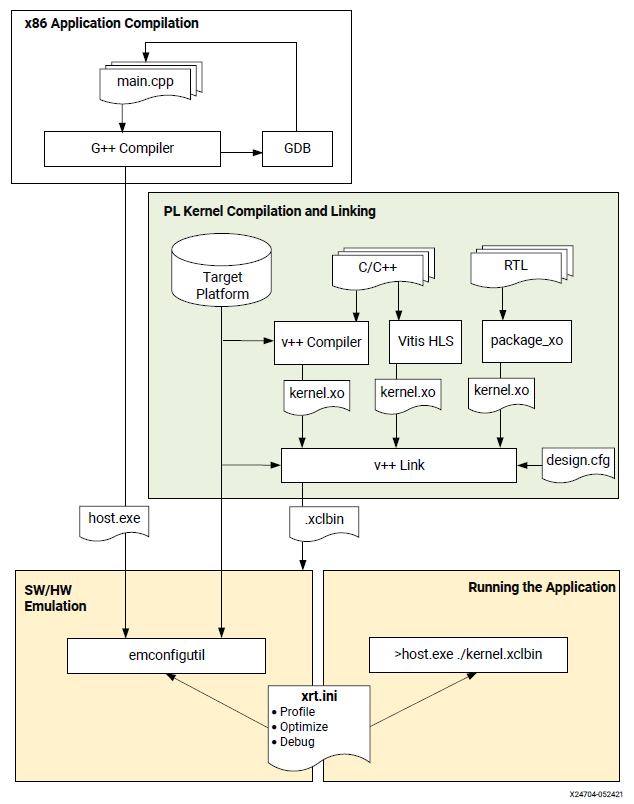
\includegraphics[width=\textwidth]{images/DataCenterFlow.PNG}
        \caption{Application Development Flow for Data Center Accelerator Cards}
        \label{DataCenterFlow}
    \end{center}
\end{figure}

\clearpage

\subsection{Embedded Processor Application Acceleration Development Flow}
The following diagram describes the steps needed to build and run an application using Arm processors and kernels running in programmable logic regions of Versal ACAP, Zynq UltraScale+ MPSoC, and Zynq-7000 SoC devices. The steps are summarized below in \figref{EmbeddedFlow}.

\begin{figure}[H]
    \begin{center}
        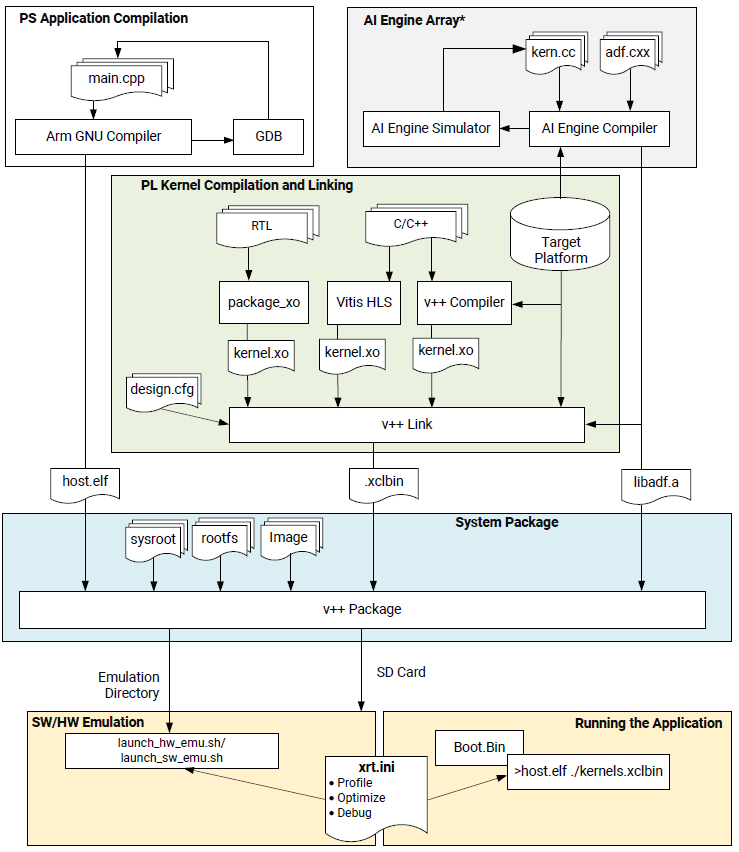
\includegraphics[width=\textwidth]{images/EmbeddedFlow.PNG}
        \caption{Application Development Flow for Versal ACAP and Zynq UltraScale+ MPSoC Devices}
        \label{EmbeddedFlow}
    \end{center}
\end{figure}

\clearpage

\begin{enumerate}
    \item PS Application Compilation: Compile the host application to run on the Cortex-A72 or Cortex-A53 core processor using the GNU Arm cross-compiler to create an ELF file. The host program interacts with kernels in the PL and AI Engine regions of the device. 
    \item  AI Engine Array (Optional for Versal AI Engine Core series only): Some Versal ACAP devices incorporate an AI Engine array of very-long instruction word (VLIW) processors with single instruction multiple data (SIMD) vector units that are highly optimized for compute-intensive applications such as 5G wireless and artificial intelligence (AI) applications. AI Engine graphs and kernels are built using Vitis tools such as the aiecompiler and aiesimulator, and can be integrated into the embedded processor application acceleration flow.
    \item  PL Kernel Compilation and Linking: PL kernels are compiled for implementation in the PL region of the target platform. PL kernels can be compiled into Xilinx object form (XO) file using the Vitis compiler (v++), Vitis HLS for C/C++ kernels, or the package\_xo command for RTL
    kernels. 
    \begin{itemize}
        \item The Vitis compiler also links the kernel XO files with the hardware platform to create a device executable (.xclbin) for the application.
        \item Xilinx object (XO) files are linked with the target hardware platform by the v++ --link command to create a device binary file (.xclbin) that is loaded into the Xilinx device on the target platform.
    \end{itemize}
    \item System Package: Use the v++ --package command to gather the required files to configure and boot the system, to load and run the application, including the host application and PL kernel binaries. This step builds the necessary package to run software or hardware emulation and debug, or to create an SD card to run your application on hardware.
    \item Running the Application: When running the application, you can run software emulation, hardware emulation, or run on the actual physical accelerator platform. Running the application on embedded processor platforms is different from running on data center accelerator cards. 
    \begin{itemize}
        \item When the build target is software or hardware emulation, the QEMU environment models the hardware device. The Vitis compiler generates simulation models of the kernels in the device binary and running the application runs in the QEMU model of the system. Emulation targets let you build, run, and iterate the design over relatively quick cycles; debugging the application and evaluating performance.
        \item When the build target is the hardware system, the target platform is the physical device. The Vitis compiler generates the .xclbin using the Vivado Design Suite to run synthesis and implementation, and resolve timing. Running the application runs your system on the hardware. The build process is automated to generate high quality results; however, hardware-savvy developers can fully leverage the Vivado tools in their design process.
    \end{itemize}
\end{enumerate}

\subsection{Build Targets}    
The Vitis compiler provides three different build targets, two emulation targets used for debug and validation purposes, and the default hardware target used to generate the actual FPGA binary:

\begin{itemize}
    \item Software Emulation (sw\_emu): Both the host application code and the kernel code are compiled to run on the host processor. This allows iterative algorithm refinement through fast build-and-run loops. This target is useful for identifying syntax errors, performing source-level debugging of the kernel code running together with application, and verifying the behavior of the system.
    \item Hardware Emulation (hw\_emu): The kernel code is compiled into a hardware model (RTL), which is run in a dedicated simulator. This build-and-run loop takes longer but provides a detailed, cycle-accurate view of kernel activity. This target is useful for testing the functionality of the logic that will go in the FPGA and getting initial performance estimates.
    \item Hardware (hw): The kernel code is compiled into a hardware model (RTL) and then implemented on the FPGA, resulting in a binary that will run on the actual FPGA.
\end{itemize}

\clearpage

\section{Methodology for Accelerating Applications with the Vitis Software Platform}
\subsection{Introduction} 
There are distinct differences between CPUs, GPUs, and programmable devices. Understanding these differences is key to efficiently developing applications for each kind of device and achieving optimal acceleration.

\par Both CPUs and GPUs have pre-defined architectures, with a fixed number of cores, a fixed instruction set, and a rigid memory architecture. GPUs scale performance through the number of cores and by employing SIMD/SIMT parallelism. In contrast, programmable devices are fully customizable architectures. The developer creates compute units that are optimized for application needs. Performance is achieved by creating deeply pipelined data-paths, rather than multiplying the number of compute units.

\begin{highlight}
    Traditional software development is about programming functionality on a pre-defined architecture. Programmable device development is about programming an architecture to implement the desired functionality.
\end{highlight}

\subsection{Methodology Overview}
The methodology is comprised of two major phases:
\begin{enumerate}
    \item Architecting the application
    \item Developing the C/C++ kernels
\end{enumerate}

In the first phase, the developer makes key decisions about the application architecture by determining which software functions should be mapped to device kernels, how much parallelism is needed, and how it should be delivered.

\par In the second phase, the developer implements the kernels. This primarily involves structuring source code and applying the desired compiler pragma to create the desired kernel architecture and meet the performance target.

\begin{figure}[H]
    \begin{center}
        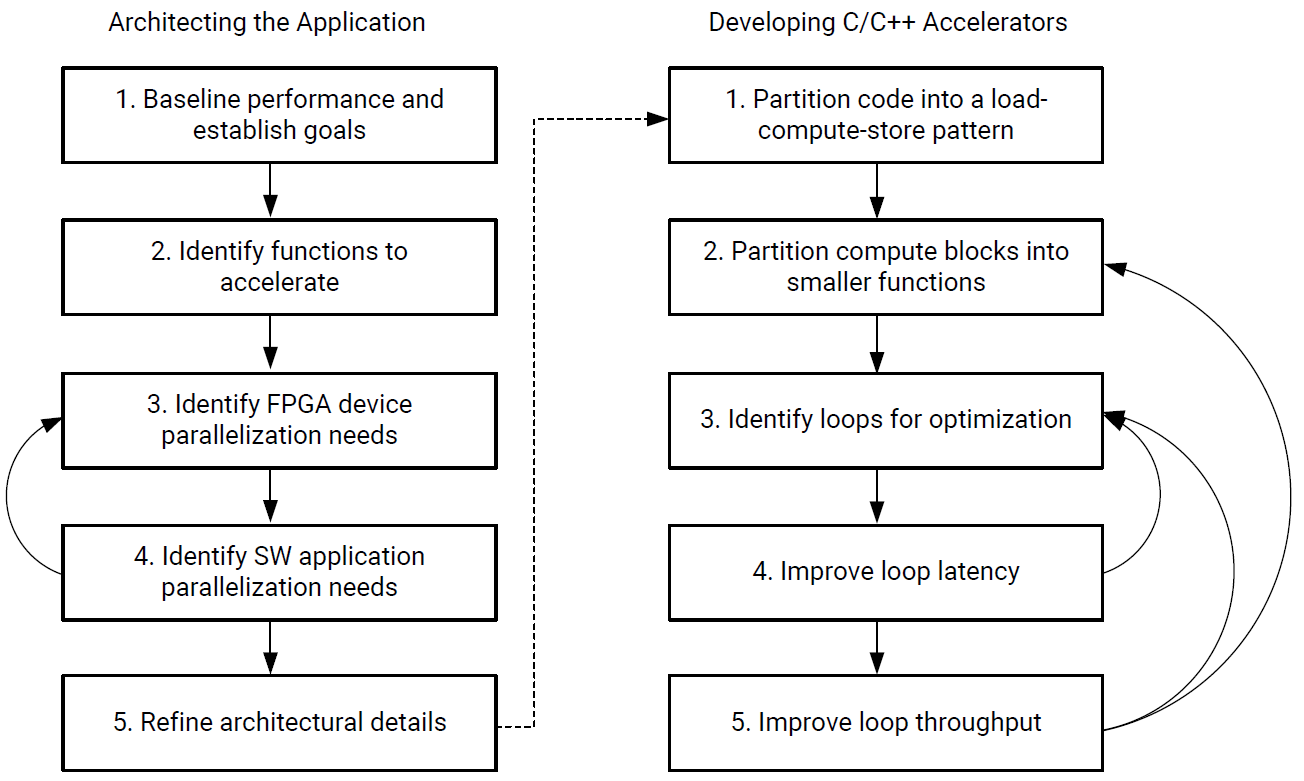
\includegraphics[width=0.75\textwidth]{images/Methodology.PNG}
        \caption{Methodology Overview}
        \label{Methodology}
    \end{center}
\end{figure}

\clearpage
\subsection{Methodology for Architecting a Device Accelerated Application}
In architecting a Device Accelerated Application phase, the developer makes key decisions about the architecture of the application and determines factors such as what software functions should be mapped to device kernels, how much parallelism is needed, and how it should be delivered.

\begin{figure}[H]
    \begin{center}
        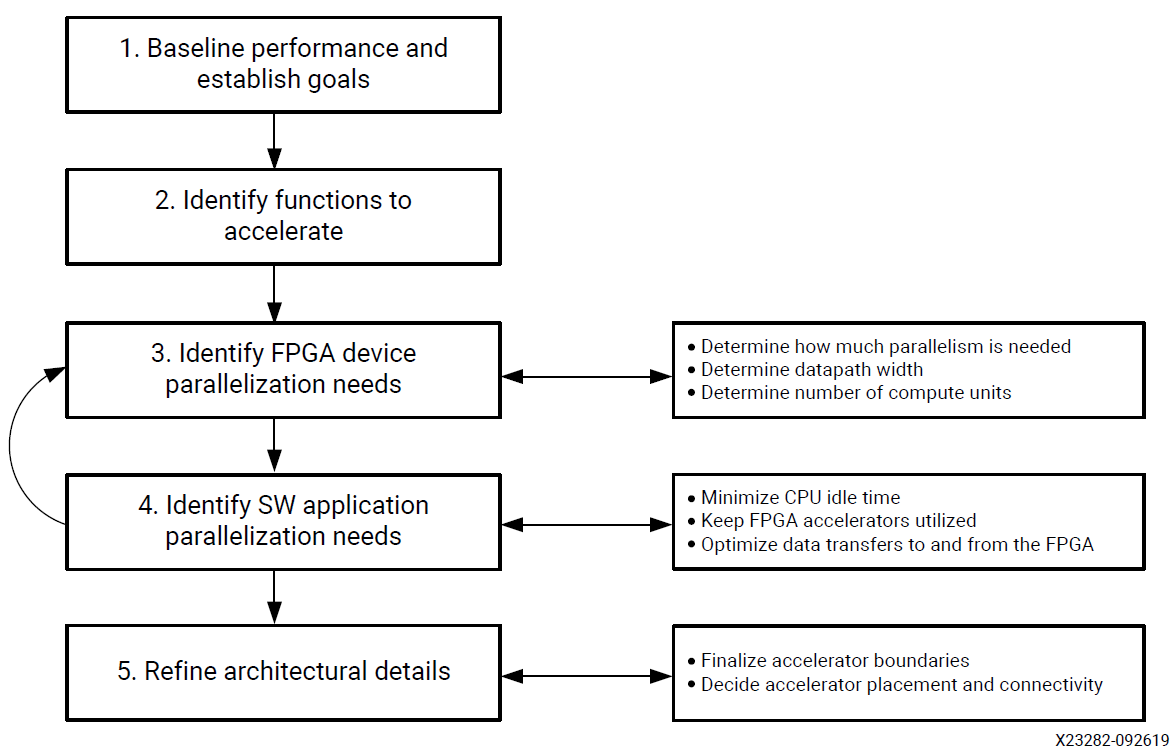
\includegraphics[width=0.75\textwidth]{images/MethodologyArchitect.PNG}
        \caption{Methodology for Architecting the Application}
        \label{MethodologyArchitect}
    \end{center}
\end{figure}

\subsubsection{Step 1: Establish a Baseline Application Performance and Establish Goals}
Start by measuring the runtime and throughput performance, to identify bottlenecks of the current application running on your existing platform. These performance numbers should be generated for the entire application (end-to-end) as well as for each major function in the application. The most effective way is to run the application with profiling tools, like valgrind, callgrind, and GNU gprof. The profiling data generated by these tools show the call graph with the number of calls to all functions and their execution time. These numbers provide the baseline for most of the subsequent analysis process. The functions that consume the most execution time are good candidates to be offloaded and accelerated onto FPGAs.

\paragraph{Measure Running Time}
Measuring running time is a standard practice in software development. This can be done using common software profiling tools such as gprof, or by instrumenting the code with timers and performance counters.

\paragraph{Measure Throughput}
Throughput is the rate at which data is being processed. To compute the throughput of a given function, divide the volume of data the function processed by the running time of the function.

\[ T_{SW} = max(V_{INPUT}, V_{OUTPUT}) / Running Time \]

Some functions process a pre-determined volume of data. In this case, simple code inspection can be used to determine this volume. In some other cases, the volume of data is variable. In this case, it is useful to instrument the application code with counters to dynamically measure the volume.

\paragraph{Determine the Maximum Achievable Throughput}
In most device-accelerated systems, the maximum achievable throughput is limited by the PCIe bus. PCIe performance is influenced by many different aspects, such as motherboard, drivers, target platform, and transfer sizes. Run DMA tests upfront to measure the effective throughput of PCIe transfers and thereby determine the upper bound of the acceleration potential, such as the xbutil dma test.

\par An acceleration goal that exceeds this upper bound throughput cannot be met as the system is I/O bound. Similarly, when defining kernel performance and I/O requirements, keep this upper bound in mind.

\paragraph{Establish Overall Acceleration Goals}
Determining acceleration goals early in the development is necessary because the ratio between the acceleration goal and the baseline performance drives the analysis and decision-making process. Acceleration goals can be hard or soft. Domain expertise is important for setting obtainable and meaningful acceleration goals.


\subsubsection{Step 2: Identify Functions to Accelerate}

\begin{highlight}
    Minimize changes to the existing code at this point so you can quickly generate a working design on the FPGA and get the baselined performance and resource numbers.
\end{highlight}

When selecting functions to accelerate in hardware, two aspects are considered:
\begin{itemize}
    \item Performance bottlenecks
    \item Acceleration potential
\end{itemize}

\paragraph{Identify Performance Bottlenecks}
In a purely sequential application, performance bottlenecks can be easily identified by looking at profiling reports. However, most real-life applications are multi-threaded and it is important to the take the effects of parallelism in consideration when looking for performance bottlenecks. When looking for acceleration candidates, consider the performance of the entire application, not just of individual functions.

\paragraph{Identify Acceleration Potential}
A function that is a bottleneck in the software application does not necessarily have the potential to run faster in a device. However, following simple guidelines can be used to assess if a function has potential for hardware acceleration:

\begin{itemize}
    \item \textbf{Computational complexity} of a function is the number of basic computing operations required to execute the function.
    \item \textbf{Computational intensity} of a function is the ratio of the total number of operations to the total amount of input and output data. Functions with a high computational intensity are better candidates for acceleration because the overhead of moving data to the accelerator is comparatively lower.
    \item \textbf{Data access locality profile:} The concepts of data reuse, spatial locality, and temporal locality are useful to assess how much overhead of moving data to the accelerator can be optimized. Spatial locality reflects the average distance between several consecutive memory access operations. Temporal locality reflects the average number of access operations for an address in memory during program execution. The lower these measures the better, because it makes data more easily cacheable in the accelerator, reducing the need to expensive and potentially redundant accesses to global memory.
    \item \textbf{How does the throughput of the function compare to the maximum achievable in a device?} The throughput of the overall application does not exceed the throughput of its slowest function. The developer can determine the maximum acceleration potential by dividing the throughput of the slowest function by the throughput of the selected function.
    \[ Maximum Acceleration Potential = T_{Min} / T_{SW} \]
    On Alveo Data Center accelerator cards, the PCIe bus imposes a throughput limit on data transfers. While it may not be the actual bottleneck of the application, it constitutes a possible upper bound and can therefore be used for early estimates.
\end{itemize}

\subsubsection{Step 3: Identify Device Parallelization Needs}
Parallelism is possibilities within kernels:
\begin{itemize}
    \item The progressive and simultaneous processing of inputs is called as pipelining.
    \item Increasing the width of the datapath within the kernel is another form of Parallelism.
\end{itemize}
The developer needs to determine which combination of parallelization techniques is most effective at meeting the acceleration goals.

\paragraph{Estimate Hardware Throughput without Parallelization}
The throughput of the kernel without any parallelization can be approximated as:
\[ T_{HW} = Frequency / Computational Intensity = Frequency * max(V_{INPUT},V_{OUTPUT}) / V_{OPS} \]
Frequency is the clock frequency of the kernel. This value is determined by the targeted acceleration platform, or target platform. The Computational Intensity of a function is the ratio of the total number of operations to the total amount of input and output data. The formula above clearly shows that functions with a high volume of operations and a low volume of data are better candidates for acceleration.

\paragraph{Determine How Much Parallelism is Needed}
The initial HW/SW performance ratio can be estimated as:
\[Speed-up = T_{HW}/T_{SW} = F_{max} * Running Time /V_{ops} \]
Without any parallelization, the initial speed-up will most likely be less than 1. To calculate how much parallelism is needed to meet the performance goal:

\[ Parallelism Needed = T_{Goal} / T_{HW} = T_{Goal} * V_{ops} / (F_{max} * max(V_{INPUT}, V_{OUTPUT})) \]

This parallelism can be implemented in various ways: by widening the datapath, by using multiple engines, and by using multiple kernel instances. The developer should then determine the best combination given their needs and the characteristics of their application.

\paragraph{Determine How Many Samples the Datapath Should be Processing
in Parallel}
One possibility is to accelerate the computation by creating a wider datapath and processing more samples in parallel. Processing more samples in parallel using a wider datapath improves performance by reducing the latency (running time) of the accelerated function.

\paragraph{Determine How Many Kernels Can and Should be Instantiated in the
Device}
If the datapath cannot be parallelized (or not sufficiently), then more kernel instances can be added. This is usually referred to as using multiple compute units (CUs). Adding more kernel instances improves the performance of the application by allowing the execution of more invocations of the targeted function in parallel. Multiple data sets are processed concurrently by the different instances. Application performance scales linearly with the number of instances, provided that the host application can keep the kernels busy.

\subsubsection{Step 4: Identify Software Application Parallelization Needs}
Parallelism in the software application can be achieved by aiming the following:
\begin{itemize}
    \item Aim to minimize CPU idle time
    \item Aim to maximize kernel utilization
    \item Aim to optimize data transfers   
\end{itemize}

\begin{figure}[H]
    \begin{center}
        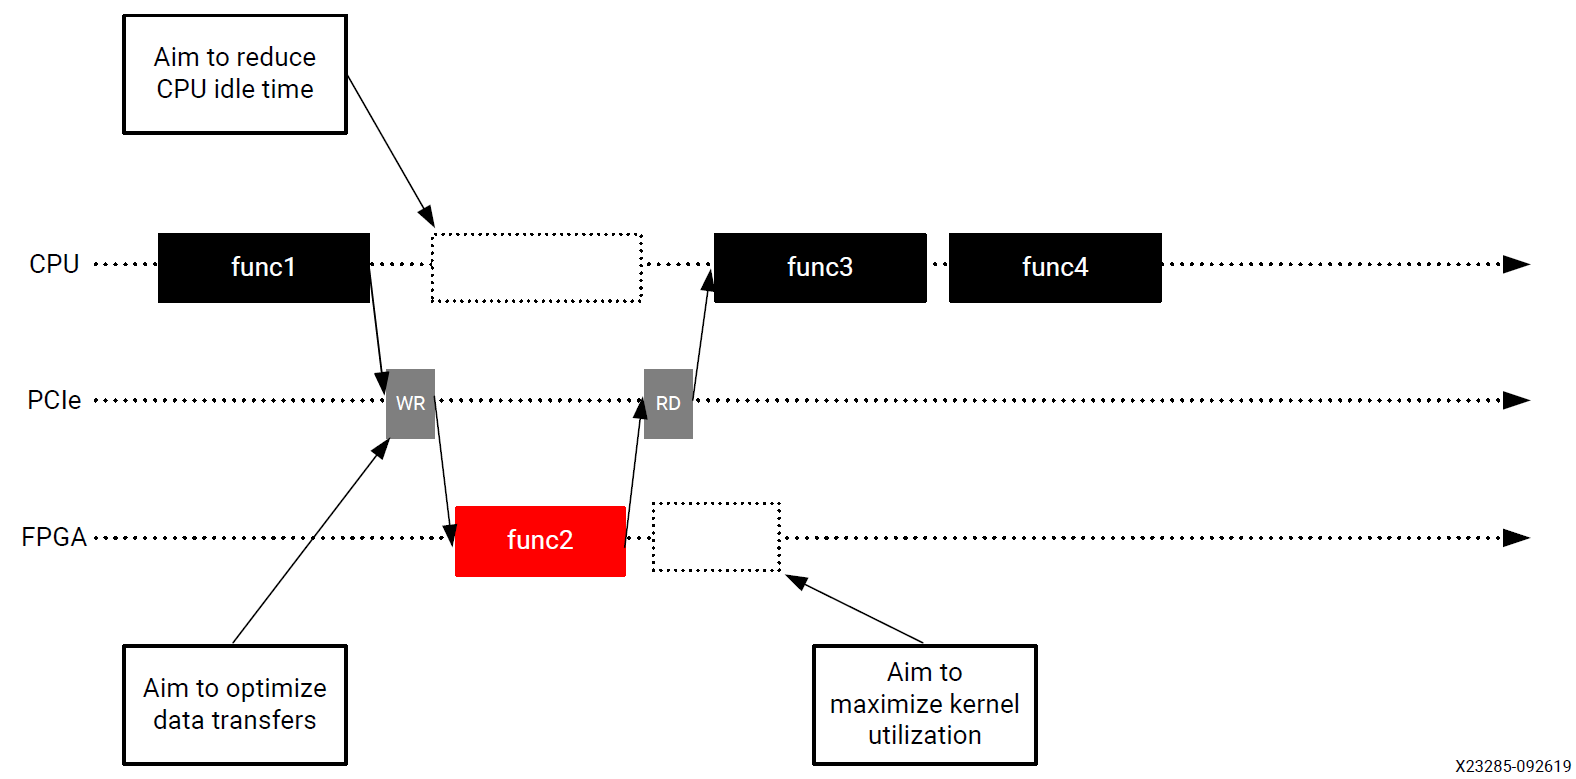
\includegraphics[width=0.9\textwidth]{images/SoftwareOptimization.PNG}
        \caption{Software Optimization Goals}
        \label{SoftwareOptimization}
    \end{center}
\end{figure}

\paragraph{Minimize CPU Idle Time While the Device Kernels are Running}
Device-acceleration is about offloading certain computations from the host processor to the kernels in the device. In a purely sequential model, the application would be waiting idly for the results to be ready and resume processing. Instead, engineer the software application to avoid such idle cycles. Begin by identifying parts of the application that do not depend on the results of the kernel. Then structure the application so that these functions can be executed on the host in parallel to the kernel running in the device. 

\paragraph{Keep the Device Kernels Utilized}
Kernels might be present in the device, but they will only run when the application requests them. To maximize performance, engineer the application so that it will keep the kernels busy. Conceptually, this is achieved by issuing the  next requests before the current ones have completed. This results in pipelined and overlapping execution, leading to kernels being optimally utilized, as shown in \figref{AcceleratorPipeline}

\begin{figure}[H]
    \begin{center}
        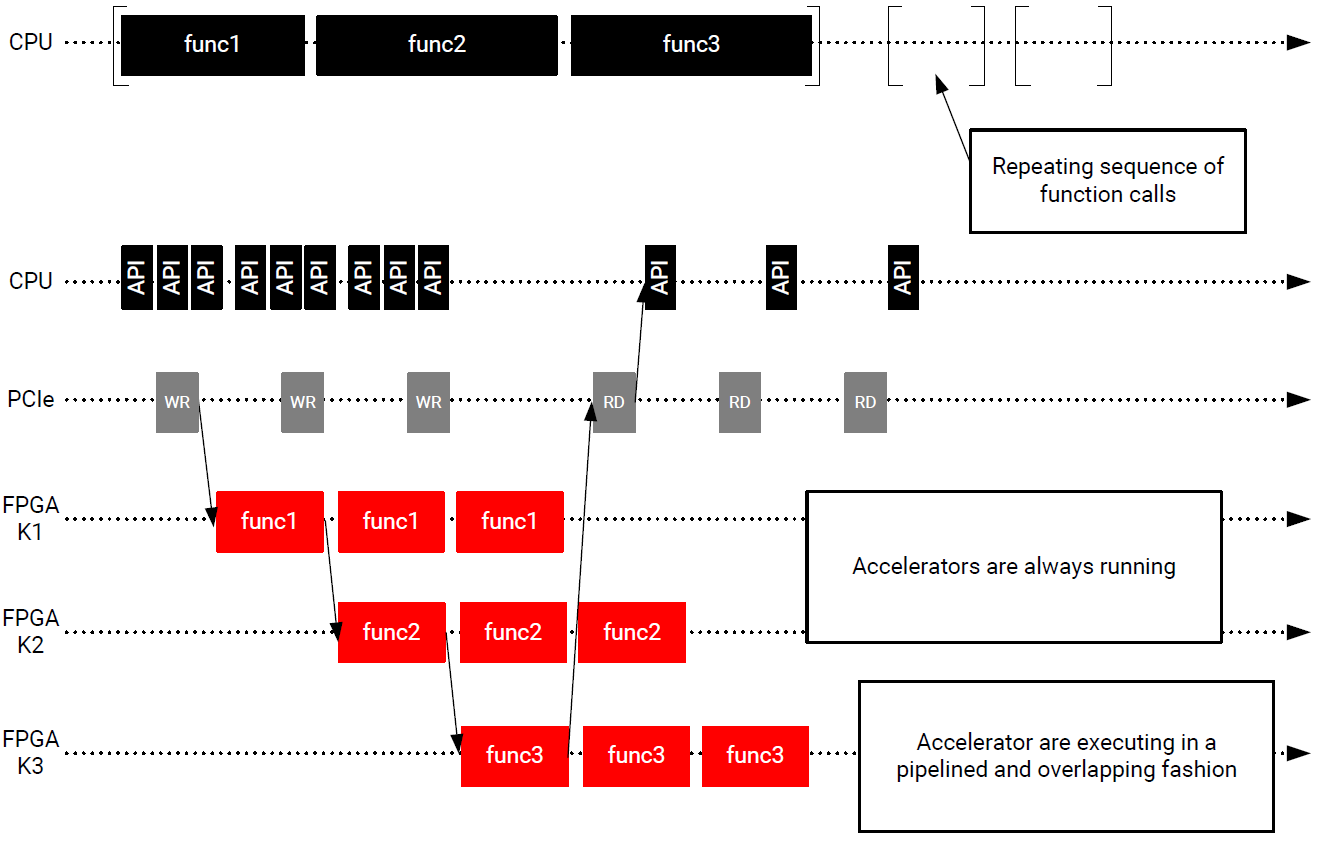
\includegraphics[width=0.9\textwidth]{images/AcceleratorPipeline.PNG}
        \caption{Pipelined Execution of Accelerators}
        \label{AcceleratorPipeline}
    \end{center}
\end{figure}

\paragraph{Optimize Data Transfers to and from the Device}
In an accelerated application, data must be transferred from the host to the device especially in the case of PCIe-based applications. This introduces latency, which can be very costly to the overall performance of the application.

\par Data needs to be transferred at the right time, otherwise the application performance is negatively impacted if the kernel must wait for data to be available. It is therefore important to transfer data ahead of when the kernel needs it. This is achieved by overlapping data transfers and kernel execution.

\par Another method of optimizing data transfers is to transfer optimally sized buffers. PCIe throughput varies greatly based on the transferred buffer size. The larger the buffer, the better the throughput, ensuring the accelerators always have data to operate on and are not wasting cycles. It is usually better to make data transfers of 1 MB or more. Running DMA tests upfront can be useful for finding the optimal buffer sizes. Also, when determining optimal buffer sizes, consider the effect of large buffers on resource utilization and transfer latency. Xilinx recommends grouping multiple sets of data in a common buffer to achieve the highest possible throughput.

\paragraph{Conceptualize the Desired Application Timeline}
The timeline sequences, as shown in \figref{AcceleratorPipeline}, are very effective ways of representing performance and parallelization in action as the application runs. The Vitis software platform generates timeline views from actual application runs which can be used to validate the user timeline, identify potential issues, and iterate and converge on the optimal results.

\subsubsection{Step 5: Refine Architectural Details}
The final step consists of refining and deriving second order architectural details from the top-level decisions.

\paragraph{Finalize Kernel Boundaries}
As discussed earlier, performance can be improved by creating multiple instances of kernels (compute units). However, adding CUs has a cost in terms of I/O ports, bandwidth, and resources. In the Vitis software platform flow, kernel ports have a maximum width of 512 bits (64 bytes) and have a fixed cost in terms of device resources. Most importantly, the targeted platform sets a limit on the maximum number of ports which can be used.

\par An alternative to scaling with multiple compute units is to scale by adding multiple engines within a kernel. This approach allows increasing performance in the same way as adding more CUs: multiple data sets are processed concurrently by the different engines within the kernel.

\par Placing multiple engines in the same kernel takes the fullest advantage of the bandwidth of the kernel's I/O ports. Putting multiple engines in a kernel also reduces the number of ports and the number of transactions to global memory that require arbitration, improving the effective bandwidth.

\par On the other hand, this transformation requires coding explicit I/O multiplexing behavior in the kernel. This is a trade-off the developer needs to make. 

\paragraph{Decide Kernel Placement and Connectivity}
At this point, it is important to understand the features of the target platform and what global memory resources are available.

\par Using multiple DDRs helps balance the data transfer loads and improve performance. This comes with a cost, however, as each DDR controller consumes device resources. Balance these considerations when deciding how to connect kernel ports to memory banks. Establishing these connections is done through a simple compiler switch, making it easy to change configurations if necessary.

\par After refining the architectural details, the developer should have all the information necessary to start implementing the kernels, and ultimately, assembling the entire application.


\clearpage
\subsection{Methodology for Developing C/C++ Kernels}
The Vitis software platform supports kernels modeled in either C/C++ or RTL (Verilog, VHDL, System Verilog). The following key kernel requirements for optimal application performance should have already been identified during the architecture definition phase:
\begin{itemize}
    \item Throughput goal
    \item Latency goal
    \item Datapath width
    \item Number of engines
    \item Interface bandwidth
\end{itemize}

These requirements drive the kernel development and optimization process. Achieving the kernel throughput goal is the primary objective, as overall application performance is predicated on each kernel meeting the specified throughput.

\par The kernel development methodology therefore follows a throughput-driven approach and works from the outside-in. This approach has two phases:
\begin{enumerate}
    \item Defining and implementing the macro-architecture of the kernel
    \item Coding and optimizing the micro-architecture of the kernel
\end{enumerate}

Before starting the kernel development process, it is essential to understand:
\begin{itemize}
    \item \textbf{Functionality} is the mathematical relationship between input parameters and output results.
    \item \textbf{Algorithm} is a series of steps for performing a specific functionality. A given functionality can be performed using a variety of different algorithms.
    \item \textbf{Architecture}, in this context, refers to the characteristics of the underlying hardware implementation of an algorithm.
\end{itemize}

You must understand that the Vitis compiler generates optimized hardware architectures from algorithms written in C/C++. However, it does not transform a particular algorithm into another one. Even if the software program can be automatically converted (or synthesized) into hardware,
achieving acceptable quality of results (QoR), requires additional work such as rewriting the software to help the HLS tool achieve the desired performance goals.

\begin{highlight}
    Because the algorithm directly influences data access locality as well as potential for computational parallelism, your choice of algorithm has a major impact on achievable performance, more so than the compiler's abilities or user specified pragmas. 
\end{highlight}


\begin{figure}[H]
    \begin{center}
        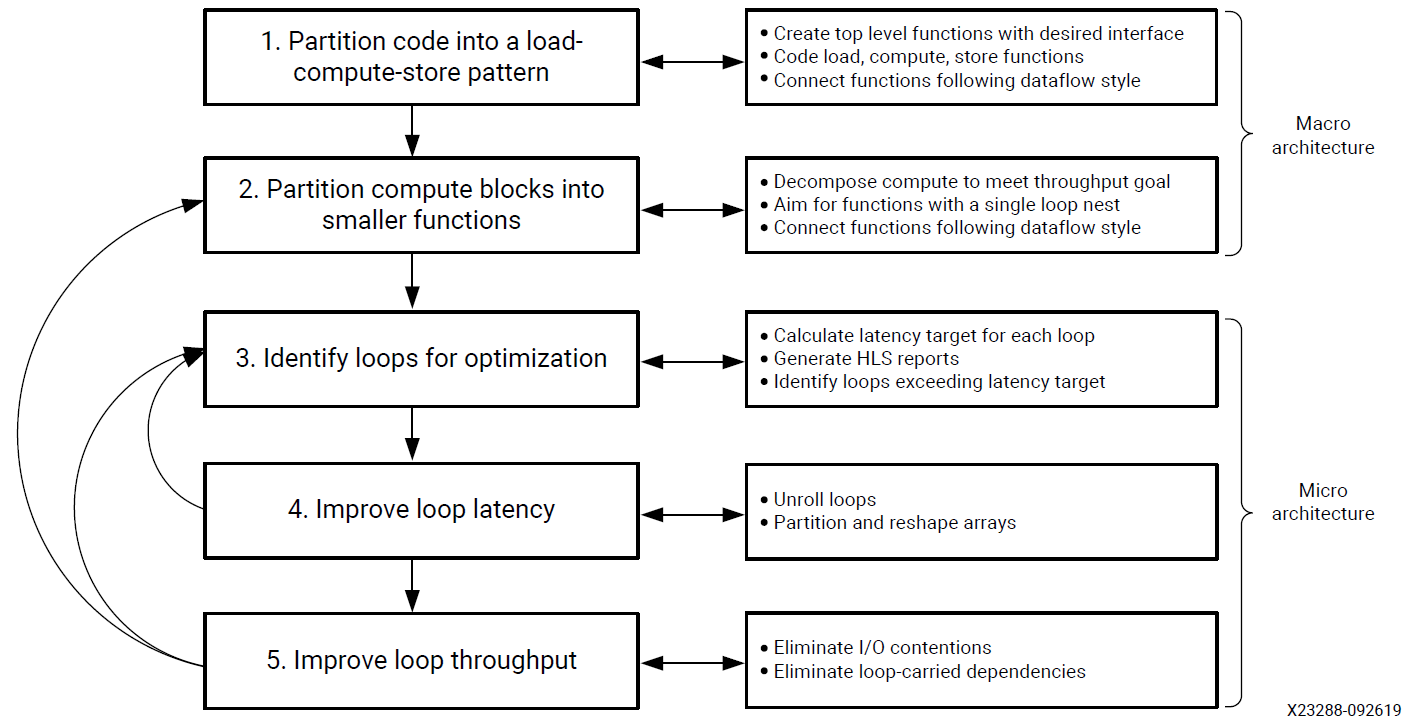
\includegraphics[width=0.9\textwidth]{images/KernelMethodology.PNG}
        \caption{Kernel Development Methodology}
        \label{KernelMethodology}
    \end{center}
\end{figure}

\subsubsection{Step 1: Partition the Code into a Load-Compute-Store
Pattern}

\begin{highlight}
    A kernel is essentially a custom datapath (optimized for the desired functionality) and an associated data storage and motion network. 
\end{highlight}

Data storage and motion network is also referred to as the memory architecture or memory hierarchy of the kernel. It is responsible for moving data in and out of the kernel and through the custom datapath as efficiently as possible.

\par Knowing that kernel accesses to global memory are expensive and that bandwidth is limited, it is very important to carefully plan this aspect of the kernel. To help with this, the first step of the kernel development methodology requires structuring the kernel code into the load-compute-store pattern. This means creating a top-level function with:

\begin{itemize}
    \item Interface parameters matching the desired kernel interface.
    \item Three sub-functions: load, compute, and store.
    \item Local arrays or hls::stream variables to pass data between these functions.
\end{itemize}

\begin{figure}[H]
    \begin{center}
        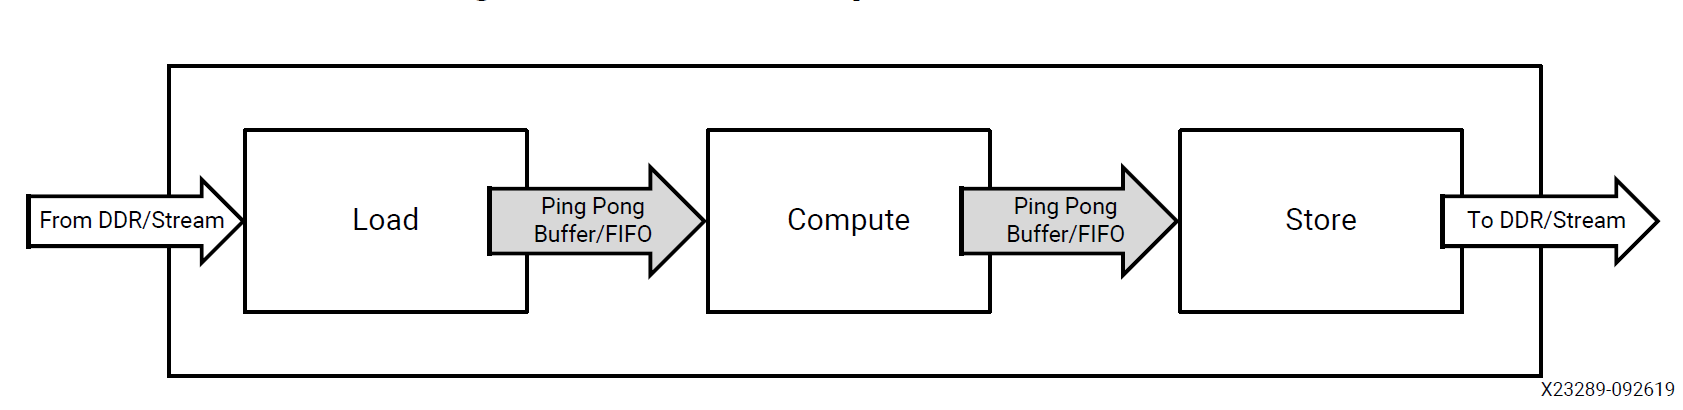
\includegraphics[width=0.9\textwidth]{images/LCSPattern.PNG}
        \caption{Load-Compute-Store Pattern}
        \label{LCSPattern}
    \end{center}
\end{figure}

Structuring the kernel code this way enables task-level pipelining, also known as HLS dataflow. This compiler optimization results in a design where each function can run simultaneously, creating a pipeline of concurrently running tasks. And this structure is key to achieving and sustaining the desired throughput. 

\begin{itemize}
    \item The \textbf{load function} is responsible for efficient data transfer (including buffering and caching if necessary) from external to the kernel (\ie global memory).
    \item The \textbf{compute function}, as its name suggests, is where all the processing is done. 
    \item The \textbf{store function} mirrors the load function. It is responsible for moving data out of the kernel, taking the results of the compute function and transferring them to global memory outside the kernel.
\end{itemize}

Understanding and visualizing the data movement as a block diagram will help to partition and structure the different functions within the kernel.

\paragraph{Create a Top-Level Function with the Desired Interface}
The Vitis technology infers kernel interfaces from the parameters of the top-level function. Therefore, it is necessary to write a kernel top-level function with parameters matching the desired interface. 

\begin{itemize}
    \item Input parameters should be passed as scalars. 
    \item Blocks of input and output data should be passed as pointers. 
    \item Compiler pragmas should be used to finalize the interface definition. 
\end{itemize}

\paragraph{Code the Load and Store Functions}
Data transfers between the kernel and global memories have a very big influence on overall system performance. If not properly done, they might throttle the kernel. The following are guidelines for improving the efficiency of data transfers in and out of the kernel.

\begin{itemize}
    \item Match Port Width to Datapath Width
    \item Use Burst Transfers
    \item Minimize the Number of Data Transfers from Global Memory
\end{itemize}

\paragraph{Code the Compute Functions}
The compute function is where all the actual processing is done. This first step of the methodology is focused on getting the top-level structure right and optimizing data movement. The priority is to have a function with the right interfaces and make sure the functionality is
correct. 

\paragraph{Connect the Load, Compute, and Store Functions}
Use standard C/C++ variables and arrays to connect the top-level interfaces and the load, compute and store functions. It can also be useful to use the hls::stream class, which models a streaming behavior.

\par Streaming is a type of data transfer in which data samples are sent in sequential order starting from the first sample. Streaming requires no address management and can be implemented with FIFOs. 

\par Key recommendations for function connections include:
\begin{itemize}
    \item Data should be transferred in the forward direction only, avoiding feedback whenever possible.
    \item Each connection should have a single producer and a single consumer.
    \item Only the load and store functions should access the primary interface of the kernel.
\end{itemize}

\subsubsection{Step 2: Partition the Compute Blocks into Smaller Functions}
The next step is to refine the main compute function, decomposing it into a sequence of smaller sub-functions, as shown in the \figref{computeSubFunctions}

\begin{figure}[H]
    \begin{center}
        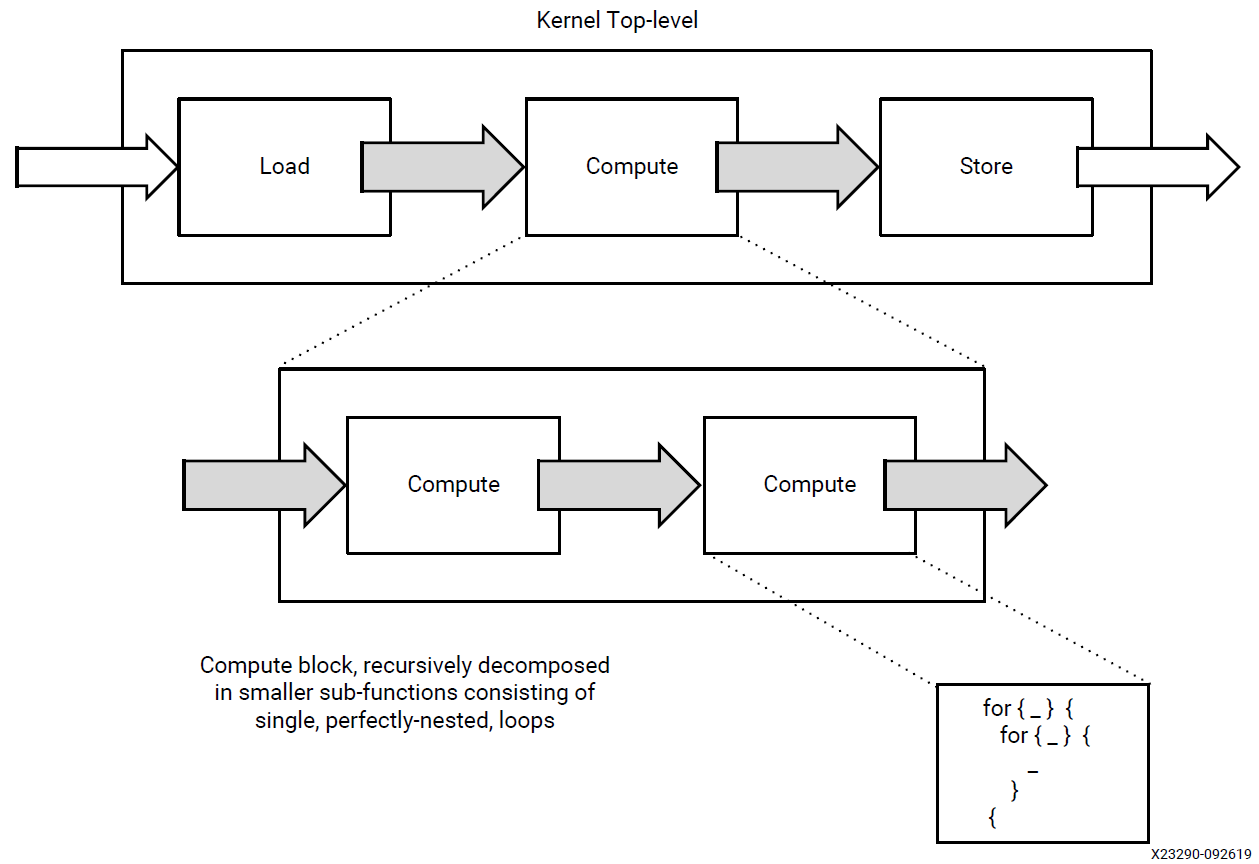
\includegraphics[width=0.9\textwidth]{images/computeSubFunctions.PNG}
        \caption{Compute Block Sub-Functions}
        \label{computeSubFunctions}
    \end{center}
\end{figure}

\paragraph{Decompose to Identify Throughput Goals}
In a dataflow system like the one created with this approach, the slowest task will be the bottleneck.

\[ Throughput(Kernel) = min(Throughput(Task1), Throughput(Task2), \dots,\]
\[ Throughput(TaskN)) \]

Therefore, during the decomposition process, always have the kernel throughput goal in mind and assess whether each sub-function will be able to satisfy this throughput goal.

\paragraph{Aim for Functions with a Single Loop Nest}
As a general rule, if a function has sequential loops in it, these loops execute sequentially in the hardware implementation generated by the HLS compiler. This is usually not desirable, as sequential execution hampers throughput.

\par However, if these sequential loops are pushed into sequential functions, then the HLS compiler can apply the dataflow optimization and generate an implementation that allows the pipelined and overlapping execution of each task. 

\par During this partitioning and refining process, put sequential loops into individual functions. Ideally, the lowest-level compute block should only contain a single perfectly-nested loop. 

\paragraph{Connect Compute Functions Using the Dataflow 'Canonical Form'}
Rules regarding connectivity while decomposing the compute function:
\begin{itemize}
    \item Aim for feed-forward connections. 
    \item Have a single producer and consumer for each connecting variable. 
    \item If a variable must be consumed by more than one function, then it should be explicitly duplicated.
    \item When moving blocks of data from one compute block to another, the developer can choose to use arrays or hls::stream objects.
\end{itemize}

Using arrays requires fewer code changes and is usually the fastest way to make progress during the decomposition process. However, using hls::stream objects can lead to designs using less memory resources and having shorter latency. It also helps the developer reason about how data
moves through the kernel, which is always an important thing to understand when optimizing for throughput.

\par At this stage, maintaining a graphical representation of the architecture of the kernel can be very useful to reason through data dependencies, data movement, control flows, and concurrency.

\subsubsection{Step 3: Identify Loops Requiring Optimization}
The throughput of a function is measured by dividing the volume of data processed by the latency, or running time, of the function.
\[ T = max(V_{INPUT}, V_{OUTPUT}) / Latency \]

The latency of a loop can be calculated as follows:
\[LatencyLoop = (Steps + II x (TripCount - 1)) x ClockPeriod \] 
Where:
\begin{itemize}
    \item \textbf{Steps}: Duration of a single loop iteration, measured in number of clock cycles
    \item \textbf{TripCount}: Number of iterations in the loop.
    \item \textbf{II}: Initiation Interval, the number of clock cycles between the start of two consecutive iterations. When a loop is not pipelined, its II is equal to the number of Steps.
\end{itemize}

Assuming a given clock period, there are three ways to reduce the latency of a loop, and thereby improve the throughput of a function:
\begin{itemize}
    \item Reduce the number of Steps in the loop (take less time to perform one iteration).
    \item Reduce the Trip Count, so that the loop performs fewer iterations.
    \item Reduce the Initiation Interval, so that loop iterations can start more often.
\end{itemize}

Assuming a trip count much larger than the number of steps, halving either the II or the trip count can be sufficient to double the throughput of the loop.

\subsubsection{Step 4: Improve Loop Latencies}
After identifying loops latencies that exceed their target, the first optimization to consider is loop unrolling.

\paragraph{Apply Loop Unrolling}
Loop unrolling unwinds the loop, allowing multiple iterations of the loop to be executed together, reducing the loop's overall trip count. Loop unrolling can widen the resulting datapath by the corresponding factor. This usually increases the bandwidth requirements as more samples are processed in parallel. This has two implications:

\begin{itemize}
    \item The width of the function I/Os must match the width of the datapath and vice versa.
    \item No additional benefit is gained by loop unrolling and widening the datapath to the point where I/O requirements exceed the maximum size of a kernel port (512 bits / 64 bytes).
\end{itemize}

Guidelines to optimize the use of loop unrolling:
\begin{itemize}
    \item Start from the innermost loop within a loop nest.
    \item Assess which unroll factor would eliminate all loop-carried dependencies.
    \item For more efficient results, unroll loops with fixed trip counts.
    \item If there are function calls within the unrolled loop, in-lining these functions can improve results through better resource sharing, although at the expense of longer synthesis times. Note also that the interconnect may become increasingly complex and lead to routing
    problems later on.
    \item Do not blindly unroll loops. Always unroll loops with a specific outcome in mind.
\end{itemize}


\paragraph{Apply Array Partitioning}
If a loop makes array accesses ensure that the resulting datapath can access all the data it needs in parallel. If unrolling a loop does not result in the expected performance improvement, this is almost always because of memory access bottlenecks.

\par Consider using various pragmas to partition and reshape arrays, when loop unrolling to create a memory structure that allows the desired level of parallel accesses.

\par Unrolling and partitioning arrays can be sufficient to meet the latency and throughput goals for the targeted loop. If so, shift to the next loop of interest. Otherwise, look at additional optimizations to improve throughput.

\subsubsection{Step 5: Improve Loop Throughput}
If loop latency  can be further impriovced by reducing the initiation interval (II). The loop II is the count of clock cycles between the start of two loop iterations. The Vitis HLS compiler will always try to pipeline loops, minimize the II, and start loop iterations as early as possible, ideally starting a new iteration each clock cycle (II=1). There are two main factors that can limit the II:
\begin{itemize}
    \item I/O contentions
    \item Loop-carried dependencies
\end{itemize}

\paragraph{Eliminate I/O Contentions}
I/O contentions appear when a given I/O port of internal memory resources must be accessed more than once per loop iteration. A loop cannot be pipelined with an II lower than the number of times an I/O resource is accessed per loop iteration. \eg If port A must be accessed four times in a
loop iteration, then the lowest possible II will be 4 in single-port RAM.

The most common techniques for reducing I/O contentions are:
\begin{itemize}
    \item Creating internal cache structures
    \item Reconfiguring I/Os and memories
\end{itemize}

\paragraph{Eliminate Loop-Carried Dependencies}
The most common case for loop-carried dependencies is when a loop iteration relies on a value computed in a prior iteration.

\begin{itemize}
    \item Eliminating dependencies on arrays: The HLS compiler performs index analysis to determine whether array dependencies exist (read-after-write, write-after-read, write-after-write). Special compiler pragmas can overwrite these dependencies and improve the II of the design.
    \item Eliminating dependencies on scalars: In the case of scalar dependencies, there is usually a feedback path with a computation scheduled over multiple clock cycles. The number of cycles in the feedback path directly limits the potential II and should be reduced to improve II and throughput. 
\end{itemize}

If an II of 1 is usually the best scenario, it is rarely the only sufficient scenario. The goal is to meet the latency and throughput goal. To this extent, various combinations of II and unroll factor are
often sufficient.


%   Section  II: Developing Applications   
\section{Programming Model}
\subsection{Device Topology}
\subsection{Kernel Properties}


\section{Host Programming}
\subsection{Specifying the Device ID and Loading the XCLBIN}
\subsection{Setting Up XRT-Managed Kernels and Kernel Arguments}
\subsection{Transferring Data between Host and Kernels}
\subsection{Executing Kernels on the Device}
\subsection{Setting Up User-Managed Kernels and Argument Buffers}
\subsection{Summary}


\section{C/C++ Kernels}
\subsection{Process Execution Modes}
\subsection{Data Types}
\subsection{Interfaces}
\subsection{Loops}
\subsection{Dataflow Optimization}
\subsection{Array Configuration}
\subsection{Function Inlining}
\subsection{Auto-Restarting Kernels}
\subsection{Summary}


\section{RTL Kernels}
\subsection{Requirements of an RTL Kernel}
\subsection{Creating User-Managed RTL Kernels}
\subsection{RTL Kernel Development Flow}
\subsection{Design Recommendations for RTL Kernels}

\section{Best Practices for Acceleration with Vitis} 



